\documentclass{beamer}
\usepackage{amsmath}
\usepackage[english]{babel} %set language; note: after changing this, you need to delete all auxiliary files to recompile
\usepackage[utf8]{inputenc} %define file encoding; latin1 is the other often used option
\usepackage{csquotes} % provides context sensitive quotation facilities
\usepackage{graphicx} %allows for inserting figures
\usepackage{booktabs} % for table formatting without vertical lines
\usepackage{textcomp} % allow for example using the Euro sign with \texteuro
\usepackage{stackengine}
\usepackage{wasysym}
\usepackage{tikzsymbols}
\usepackage{textcomp}
% ELIMINAR COMANDOS DE NAVEGACION%%%%%%%%%%%
\setbeamertemplate{navigation symbols}

%\newcommand{\bubblethis}[2]{
 %       \tikz[remember picture,baseline]{\node[anchor=base,inner sep=0,outer sep=0]%
 %       (#1) {\underline{#1}};\node[overlay,cloud callout,callout relative pointer={(0.2cm,-0.7cm)},%
 %       aspect=2.5,fill=yellow!90] at ($(#1.north)+(-0.5cm,1.6cm)$) {#2};}%
 %   }%
%\tikzset{face/.style={shape=circle,minimum size=4ex,shading=radial,outer sep=0pt,
 %       inner color=white!50!yellow,outer color= yellow!70!orange}}

%% Some commands to make the code easier
\newcommand{\emoticon}[1][]{%
  \node[face,#1] (emoticon) {};
  %% The eyes are fixed.
  \draw[fill=white] (-1ex,0ex) ..controls (-0.5ex,0.2ex)and(0.5ex,0.2ex)..
        (1ex,0.0ex) ..controls ( 1.5ex,1.5ex)and( 0.2ex,1.7ex)..
        (0ex,0.4ex) ..controls (-0.2ex,1.7ex)and(-1.5ex,1.5ex)..
        (-1ex,0ex)--cycle;}
\newcommand{\pupils}{
  %% standard pupils
  \fill[shift={(0.5ex,0.5ex)},rotate=80] 
       (0,0) ellipse (0.3ex and 0.15ex);
  \fill[shift={(-0.5ex,0.5ex)},rotate=100] 
       (0,0) ellipse (0.3ex and 0.15ex);}

\newcommand{\emoticonname}[1]{
  \node[below=1ex of emoticon,font=\footnotesize,
        minimum width=4cm]{#1};}
\usepackage{scalerel}
\usetikzlibrary{positioning}
\usepackage{xcolor,amssymb}
\newcommand\dangersignb[1][2ex]{%
  \scaleto{\stackengine{0.3pt}{\scalebox{1.1}[.9]{%
  \color{red}$\blacktriangle$}}{\tiny\bfseries !}{O}{c}{F}{F}{L}}{#1}%
}
\newcommand\dangersignw[1][2ex]{%
  \scaleto{\stackengine{0.3pt}{\scalebox{1.1}[.9]{%
  \color{red}$\blacktriangle$}}{\color{white}\tiny\bfseries !}{O}{c}{F}{F}{L}}{#1}%
}
\usepackage{fontawesome} % Social Icons
\usepackage{epstopdf} % allow embedding eps-figures
\usepackage{tikz} % allows drawing figures
\usepackage{amsmath,amssymb,amsthm} %advanced math facilities
\usepackage{lmodern} %uses font that support italic and bold at the same time

\usepackage{tikz}

\usepackage{tcolorbox}

\usefonttheme[onlymath]{serif} %set math font to serif ones

\definecolor{beamerblue}{rgb}{0.2,0.2,0.7} %define beamerblue color for later use

%%% defines highlight command to set text blue
\newcommand{\highlight}[1]{{\color{blue}{#1}}}


%%%%%%% commands defining backup slides so that frame numbering is correct

\newcommand{\backupbegin}{
   \newcounter{framenumberappendix}
   \setcounter{framenumberappendix}{\value{framenumber}}
}
\newcommand{\backupend}{
   \addtocounter{framenumberappendix}{-\value{framenumber}}
   \addtocounter{framenumber}{\value{framenumberappendix}}
}

%%%% end of defining backup slides

%Specify figure caption, see also http://tex.stackexchange.com/questions/155738/caption-package-not-working-with-beamer
\setbeamertemplate{caption}{\insertcaption} %redefines caption to remove label "Figure".
%\setbeamerfont{caption}{size=\scriptsize,shape=\itshape,series=\bfseries} %sets figure  caption bold and italic and makes it smaller


\usetheme{Boadilla}

\usepackage{hyperref}

% --------------------
% Overall information
% --------------------
\title[Economía I]{Economía I \vspace{4mm}
\\ Magistral 7: Las ganancias del comercio}
\date{}
\author[Riottini]{Franco Riottini}
\vspace{0.4cm}
\institute[]{Universidad de San Andrés} 



\begin{document}

\begin{frame}
\titlepage
\centering

\includegraphics[scale=0.2]{../Figures/logoUDESA.jpg} 
\end{frame}


\begin{frame}
\frametitle{¿Qué sucede cuando interactuamos con otros?}
\begin{itemize}
    \item En los modelos que vimos hasta ahora, las decisiones de los individuos no dependían de las decisiones de otros.
    \item Pero, ¡todo el tiempo interactuamos con otros seres humanos!
    \item La interacción genera distintos tipos de consecuencias, que afectan las decisiones de los demás individuos.
    \item ¿De qué modo la interacción afecta a los individuos? 
\end{itemize} 
\end{frame}

\begin{frame}
\frametitle{Especialización}
    \begin{itemize}
    \item ¿Conocen la historia de Robinson Crusoe?
    \item ¿Qué sucede cuando aparece Viernes?  
    \end{itemize}
    \centering \vspace{4mm}
    \begin{tabular}{|c|c|c|} \hline
        & Robinson Crusoe & Viernes \\ \hline
     Pescados   & 4 & 3 \\ \hline
     Cocos   & 6 & 2 \\ \hline     \end{tabular}
    \begin{itemize}\vspace{4mm}
    \item ¿Qué sucede si quieren consumir 6 pescados y 6 cocos por día? 
    \item ¿Les conviene especializarse?  
    \end{itemize}
\end{frame}

\begin{frame}
\frametitle{Especialización}
\begin{itemize}
    \item Costo de oportunidad de Robinson...
        \begin{itemize}
        \item De pescar en vez de recolectar cocos: $ 6/4 = 1,5 $ cocos por pescado 
        \item De recolectar cocos en vez de pescar: $ 4/6 = 2/3=0,66 $ pescados por coco
        \end{itemize}
    \item Costo de oportunidad de Viernes...
        \begin{itemize}
        \item De pescar en vez de recolectar cocos: $ 2/3 = 0,66 $ cocos por pescado
        \item De recolectar cocos en vez de pescar: $ 3/2 = 1,5 $ pescados por coco
        \end{itemize}
    \item Para ver las ventajas del comercio y la especialización debemos comparar los costos de oportunidad de los bienes entre los individuos
\end{itemize}
\end{frame}

\begin{frame}
\frametitle{Especialización}
\begin{itemize}
    \item Costo de oportunidad de pescar en vez de recolectar cocos:
        \begin{itemize}
        \item Viernes: $ 2/3 < 1,5 $ Robinson 
        \end{itemize}
    \item Costo de oportunidad de recolectar cocos en vez de pescar:
        \begin{itemize}
        \item Viernes: $ 1,5 > 2/3 $ Robinson 
        \end{itemize}
    \item Si se especializan Robinson puede trabajar media hora menos y Viernes 1 hora menos que en el caso de no especialización. 
\end{itemize}
\end{frame}

\begin{frame}
    \frametitle{Especialización}
    \begin{itemize}
        \item La división del trabajo (o especialización) permite aumentar la producción.
        \item Aprovechar la especialización es la clave del crecimiento económico (mundial).
        \item  Explica los beneficios de la globalización.
    \item Pero ¿por qué difieren las productividades?

        \begin{itemize}\vspace{2mm}
            \item Heterogeneidad y ventaja comparativa (agentes difieren en habilidades o recursos, lo que los hace más o menos productivos en una actividad particular)
            \item Learning-by-doing (desarrollo de habilidades cuando se produce algo) \vspace{2mm}
            \item Economías de escala (producir en grandes cantidades suele ser más costo-efectivo) \vspace{2mm}
        
        \end{itemize}
            \item El estudio de los incentivos para el cambio tecnológico es un área importante de estudio para la economía
    \end{itemize} 
\end{frame}

\begin{frame}
    \frametitle{Un modelo Ricardiano simple}
    \begin{itemize}
        \item 2 países: Inglaterra y Portugal\vspace{2mm}
        \item Dos productos: vino y telas\vspace{2mm}
        \item Portugal tiene la ventaja absoluta en ambos. \\
        Inglaterra puede producirlos, pero Portugal tiene condiciones favorables tanto para producir uvas (para hacer el vino), como para criar ovejas (que dan la lana para las telas)\vspace{2mm}
        \item Para Inglaterra es relativamente más difícil producir vino\vspace{2mm}
        \item Inglaterra tendrá una ventaja comparativa en la tela y se la exportará a Portugal
    \end{itemize} 
\end{frame}

\begin{frame}
    \frametitle{Un modelo Ricardiano simple}
    \begin{itemize}
        \item Supongamos que en Portugal (P) e Inglaterra (I) los bienes se producen sólo con trabajo (L), los trabajadores de cada país son:
            \begin{center}
                $L_P=25$
                $L_I=100$
            \end{center}

            \item La productividad marginal del trabajo... 
            \begin{itemize}
                \item ... en Portugal un trabajador puede producir 4 botellas de vino o 2 metros de tela \\\vspace{2mm}
                \begin{center}
                    $PMgL_V = 4$ y $PMgL_t = 2$
                \end{center}
                \item ... en Inglaterra un trabajador puede producir 1 botella de vino o 1 metro de tela \\\vspace{2mm}
                \begin{center}
                    $PMgLv = 1$ y $PMgLt = 1$
                \end{center}
            \end{itemize} 
        \item ¿Cuáles son las posibilidades de producción?    
    \end{itemize} 
\end{frame}

\begin{frame}
\frametitle{Portugal}
\centering
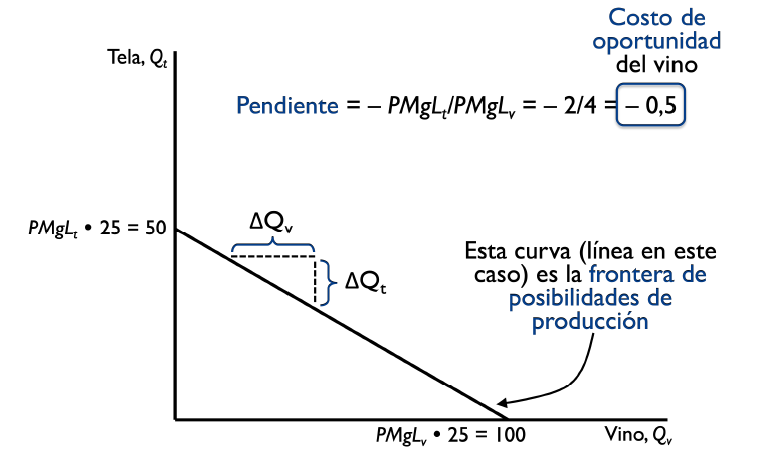
\includegraphics[scale=0.6]{../Figures/Tema_03_1_portugal.png}
\end{frame}

\begin{frame}
\frametitle{Eligiendo en Portugal}
\centering
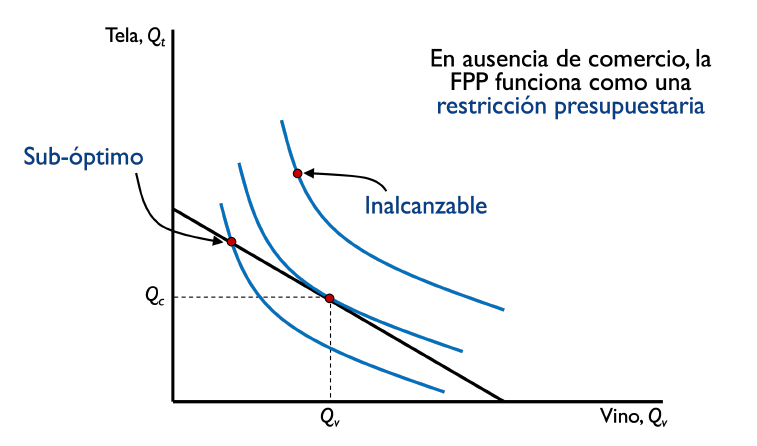
\includegraphics[scale=0.6]{../Figures/Tema_03_2_portugal2.png}
\end{frame}

\begin{frame}
\frametitle{Inglaterra}
\centering
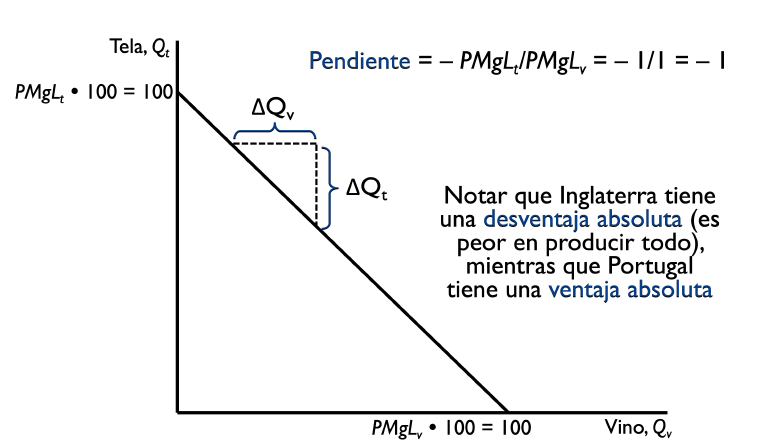
\includegraphics[scale=0.6]{../Figures/Tema_03_3_inglaterra.png}
\end{frame}

\begin{frame}
\frametitle{Eligiendo en Inglaterra}
\centering
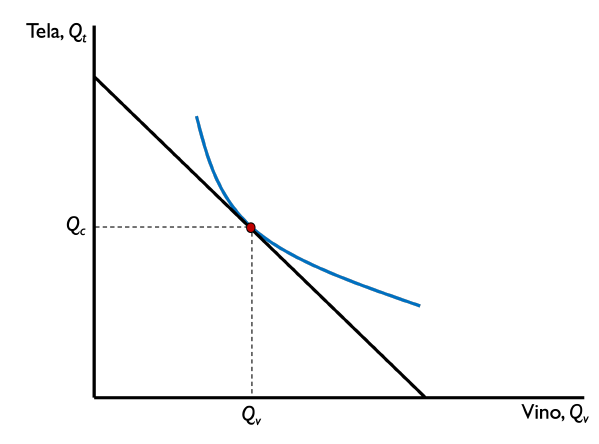
\includegraphics[scale=0.6]{../Figures/Tema_03_4_inglaterra2.png}
\end{frame}

\begin{frame}
\frametitle{Ventaja comparativa}
\begin{itemize}
    \item El costo de oportunidad varía entre los distintos países\vspace{2mm}
    \begin{itemize}
        \item En Inglaterra le toma 1 trabajador producir 1 metro de tela o una botella de vino...\vspace{2mm}
        \item ... pero en Portugal un trabajador produce 2 metros de tela o 4 botellas de vino\vspace{4mm}
    \end{itemize}
    \item Inglaterra tiene una ventaja comparativa en producir tela
    \begin{itemize}\vspace{2mm}
        \item El costo de oportunidad de la tela (1 botella de vino) es menor que en Portugal (2 botellas de vino)\vspace{2mm}
        \item El precio relativo del vino en Inglaterra es mayor que en Portugal
    \end{itemize}
\end{itemize}
\end{frame}

\begin{frame}
\frametitle{Mercado y comercio}
\begin{itemize}
    \item Cada país va a exportar el bien en el cual tiene una ventaja comparativa\vspace{4mm}
    \item Portugal exportará vino, Inglaterra tela\vspace{2mm}
        \begin{itemize}
        \item Productores en Portugal, donde $Pv/Pt = 0,5$ van a querer producir y exportar vino a Inglaterra, donde $Pv/Pt = 1$\vspace{2mm}
        \item Productores en Inglaterra, donde $Pt/Pv = 1$ van a querer producir y exportar tela a Portugal, donde $Pt/Pv = 2$\vspace{2mm}
        \item Los precios de exportación van a subir, mientras que los precios de importación van a bajar
        \end{itemize}
\end{itemize}
\end{frame}

%\begin{frame}
%\frametitle{Mercado y comercio}
%\begin{itemize}
%    \item El costo de oportunidad de la tela (1 botella de vino) es menor que en Portugal (2 botellas de vino)
%    \item El precio relativo del vino en Inglaterra es mayor que en Portugal
%\end{itemize}
%\end{frame}

\begin{frame}
\frametitle{Portugal cuando comercia}
\centering
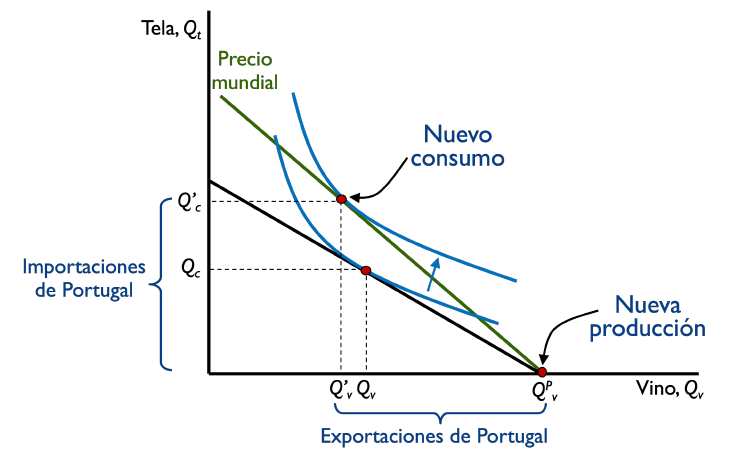
\includegraphics[scale=0.6]{../Figures/Tema_03_5_portugal3.png}
\end{frame}

\begin{frame}
\frametitle{Inglaterra cuando comercia}
\centering
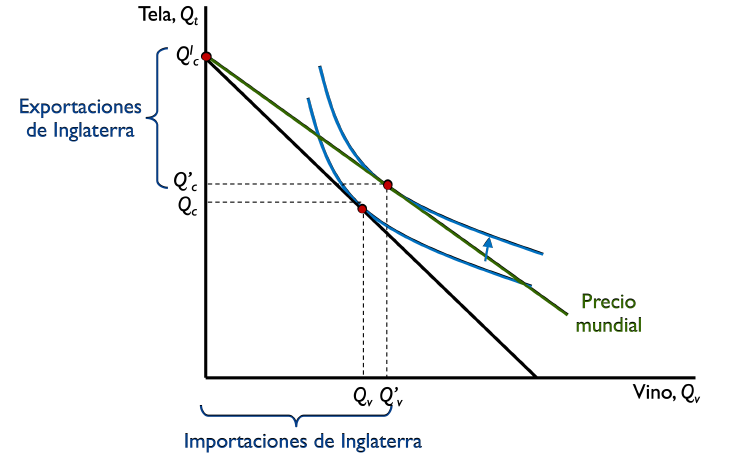
\includegraphics[scale=0.6]{../Figures/Tema_03_6_inglaterra3.png}
\end{frame}

\begin{frame}
\frametitle{Conclusiones}
\begin{itemize}
    \item La presencia de mercados logra algo notable: cooperación no intencionada entre extraños\vspace{4mm}
    \item El libre comercio ejemplifica un juego en el que todos los participantes pueden beneficiarse de un escenario en el que todos ganan, todos cooperan para alcanzar el beneficio máximo \vspace{4mm}
    \item Esto es lo contrario de un juego de suma cero\vspace{2mm}
    \begin{itemize}
      \item Los pagos totales para todos los jugadores en el juego suman cero\vspace{2mm}
    \item La ganancia de un jugador será exactamente igual a la pérdida del otro jugador\vspace{2mm}
  \item La economía es la ciencia del "win-win". 
    \end{itemize}
    
\end{itemize}
\end{frame}

\begin{frame}
\frametitle{A veces, por distintos motivos, la interacción social puede generar desvíos}
\begin{itemize}
    \item Una parte de la economía estudia este tipo de dilemas sociales\vspace{4mm}
     \item Parte de estos problemas que surgen en un mercado los vamos a estudiar más adelante\vspace{4mm}
    \item Para modelar cuando ocurren como resultado de interacciones individuales se suele utilizar lo que se conoce como teoría de juegos
    \end{itemize}
\end{frame}


\end{document}




%%%%%%%%%%%%%%%%%%%%%%%%%%%%%%%%%%%%%%%%%%%%%%%%%%%%%%%%%%%%%%%%%%%%%%%%%
\begin{frame}
\frametitle{Teoría de juegos}
\begin{itemize}
\item Estudia de manera formal y abstracta las decisiones óptimas que deben tomar diversos adversarios en conflicto.\vspace{4mm}
\item Es el estudio matemático de la toma de decisiones, del conflicto y la estrategia en situaciones sociales.\vspace{4mm}
\item Los jugadores toman decisiones que se consideran estratégicas\vspace{2mm}
    \begin{itemize}
        \item los jugadores son entes racionales (no necesariamente humanos)\vspace{2mm}
        \item los entes que participan en el juego actúan teniendo en cuenta las acciones que tomarían los demás
            \end{itemize}
\end{itemize}
\end{frame}


\begin{frame}
\frametitle{Elementos de un juego}
\begin{itemize}
\item \textbf{Los jugadores:} quién está interactuando con quién.\vspace{4mm}
\item \textbf{Las estrategias viables:} qué acciones están abiertas a los jugadores.\vspace{4mm}
\item \textbf{La información:} lo que cada jugador sabe al tomar su decisión.\vspace{4mm}
\item \textbf{Los beneficios:} cuáles serán los resultados para cada una de las posibles combinaciones de acciones.\vspace{4mm}
\end{itemize}
\end{frame}

\begin{frame}
\frametitle{Tipos de juegos}
\begin{itemize}
\item Juegos simultáneos: donde se toma una decisión one-shot.\vspace{4mm}
\item Juegos secuenciales: donde los jugadores toman sus decisiones de forma consecutiva.\vspace{4mm}
\item Juego de información perfecta: donde los individuos conocen las reglas del juego.\vspace{4mm}
\item  Juegos de información completa: donde los individuos conocen las movidas que hicieron los otros jugadores.\vspace{4mm}
\item  Juegos de información incompleta: donde los individuo no conocen la historia.
\end{itemize}
\end{frame}


%\begin{frame}
%\frametitle{Estudiando juegos}
%\begin{itemize}
%\item El término ``juegos'' refiere básicamente a modelos de interacción estratégica
%\begin{itemize}
%    \item Es decir, modelos donde las personas involucradas en una interacción social saben que sus acciones afectan a otros y viceversa
  
 %       \item En este contexto, una estrategia es una acción (o un curso de acción) que puede tomar una persona cuando es consciente de esta dependencia mutua de los resultados
   
%\end{itemize}

%\end{itemize}
%\end{frame}




\begin{frame}
\frametitle{23. Juegos simultáneos}
\begin{itemize}
\item En los juegos simultáneos, cada jugador decide su estrategia antes de conocer las decisiones de otros jugadores
\item Para analizar estos juegos, usamos la matriz o forma estratégica de un juego
\item La combinación de las estrategias elegidas por los jugadores determina la ganancia de cada jugador
\end{itemize}
\end{frame}


\begin{frame}
\frametitle{25. Dilema del prisionero}
\begin{itemize}
\item Dos sospechosos son arrestados y acusados de un delito
\item La policía no tiene evidencia suficiente para condenar a los sospechosos a menos que uno confiese
\item La policía encierra a los sospechosos en celdas separadas y les explica las consecuencias derivadas de las decisiones que formen
\end{itemize}
\end{frame}

\begin{frame}
\frametitle{26. Dilema de los prisioneros}
\begin{itemize}
\item Si ninguno confiesa, ambos serán condenados por un delito menor sentenciados a un mes de cárcel
\item Si ambos, confiesan serán sentenciados a seis meses de cárcel
\item Finalmente, si uno confiesa y el otro no, el que confiesa será puesto en libertad inmediatamente y el otro
será sentenciado a nueve meses en prisión, seis por el delito y tres más por obstrucción a la justicia
\end{itemize}
\end{frame}

\begin{frame}
\frametitle{27. Dilema de los prisioneros}
\begin{table}
     \begin{tabular}{cc|c|c|}
      & \multicolumn{1}{c}{} & \multicolumn{2}{c}{Preso $2$}\\
      & \multicolumn{1}{c}{} & \multicolumn{1}{c}{No confesar}  & \multicolumn{1}{c}{Confesar} \\\cline{3-4}
      \multirow{}{Preso $1$}  & No Confesar & $(-1,-1)$ & $(-9,0)$ \\\cline{3-4}
      & Confesar & $(0,-9)$ & $(-6,-6)$ \\\cline{3-4}
    \end{tabular}
  \end{table}
\end{frame}

\begin{frame}
\frametitle{28. Dilema de los prisioneros}
\begin{itemize}
\item Cada jugador cuenta con dos estrategias posibles: confesar y no confesar. 
\item Las ganancias de los dos jugadores cuando eligen un par concreto de estrategias aparecen en la casilla correspondiente de la matriz binaria. 
\item Por convención, la ganancia del llamado jugador-fila (Preso 1) es la primera ganancia, seguida, por la ganancia del jugador columna (Preso 2). 
\end{itemize}
\end{frame}

\begin{frame}
\frametitle{29. Dilema de los prisioneros}
\begin{itemize}
\item Por ejemplo, el preso 1 elige no confesar y el preso 2 elige confesar, el preso 1 recibe una ganancia de -9 (que representa nueve meses en prisión) y el preso 2 recibe una ganancia de 0 (que representa la inmediata puesta en libertad).
\item La representación en forma normal de un juego especifica: 
\begin{enumerate}
\item [1] los jugadores en el juego,
\item [2] las estrategias de que dispone cada jugador, y 
\item [3] la ganancia de cada jugador en cada combinación posible de estrategias.
\end{enumerate}
\end{itemize}
\end{frame}







$$$$$$$$$$$$$$
\begin{frame}
\frametitle{22. Teoría de juegos y estrategia competitiva}
\begin{block}{Equilibrio de Nash}
Un equilibrio de Nash es un par de estrategias, una para cada jugador, en las que cada estrategia es la mejor respuesta dado lo que hace el otro
\end{block}
\vspace{5mm}
En equilibrio, cada jugador está haciendo lo mejor que puede, dado lo que el otro jugador también lo está haciendo
\end{frame}
$$$$$$$$$$$$$$$$$$